% options:
% thesis=B bachelor's thesis
% thesis=M master's thesis
% czech thesis in Czech language
% english thesis in English language
% hidelinks remove colour boxes around hyperlinks

\documentclass[thesis=M,english]{FITthesis}[2012/10/20]

\usepackage[utf8]{inputenc} % LaTeX source encoded as UTF-8

\usepackage{graphicx} %graphics files inclusion
% \usepackage{subfig} %subfigures
% \usepackage{amsmath} %advanced maths
% \usepackage{amssymb} %additional math symbols

\usepackage{listings}
\usepackage{dirtree} %directory tree visualisation
\usepackage{tablefootnote}
\usepackage{subcaption}

\usepackage{pifont}% http://ctan.org/pkg/pifont
\newcommand{\cmark}{\ding{51}}%
\newcommand{\xmark}{\ding{55}}%

% list of acronyms
% \usepackage[acronym,nonumberlist,toc,numberedsection=autolabel,nomain]{glossaries}
%\iflanguage{czech}{\renewcommand*{\acronymname}{Seznam pou{\v z}it{\' y}ch zkratek}}{}
% \makeglossaries

\newcommand{\tg}{\mathop{\mathrm{tg}}} %cesky tangens
\newcommand{\cotg}{\mathop{\mathrm{cotg}}} %cesky cotangens

\graphicspath{ {images/} }

% % % % % % % % % % % % % % % % % % % % % % % % % % % % % % % % % % % 
% % % % % % % % % % % % % % % % % % % % % % % % % % % % % % % % % % % 
\department{Department of Computer Systems}
\title{TODO}
\authorGN{Tom{\' a}{\v s}} %author's given name/names
\authorFN{Su{\v s}{\' a}nka} %author's surname
\author{Tom{\' a}{\v s} Su{\v s}{\' a}nka} %author's name without academic degrees
\authorWithDegrees{Bc. Tom{\' a}{\v s} Su{\v s}{\' a}nka} %author's name with academic degrees
\supervisor{Ing. Josef Kokeš}
\acknowledgements{TODO}
\abstractCS{TODO}
\abstractEN{TODO}
\placeForDeclarationOfAuthenticity{Prague} %where you have signed the declaration
\keywordsCS{TODO}
\keywordsEN{TODO}
\declarationOfAuthenticityOption{4} %select as appropriate, according to the desired license TODO

\begin{document}

% \newacronym{IM}{IM}{Instant Messanger}
% \newacronym{RLE}{RLE}{Run-Length Encoding}

\begin{introduction}
TODO
\end{introduction}



\chapter{Current security status of major IMs}\label{compar}

This chapter contains thorough description of five selected Instant Messengers and its security related findings. Particular software versions are mostly an estimate based on a date some findings were published and the software changelog.

\section{Selection}

We selected the following five Instant Messenger applications. The selection was based on various criterions to create a diverse mixture of messengers. The criterions included user base, geographical origin, authors, proclaimed security, license, price and other. For ease of comparison we've decided to select messengers with support for mobile platforms. We've omitted Facebook Messenger, since it is owned by the very same company as WhatsApp, Facebook Inc \cite{facebookwhatsappbuy}.

\subsection{WhatsApp\protect\footnote{https://www.whatsapp.com}}

Large user base and overall popularity of the application is one of the main reasons WhatsApp is included. With 1 billion active users it is the most used messenger at the moment.\cite{whatsappusers}

\subsection{Telegram\protect\footnote{https://www.telegram.org}}

Telegram praises itself as safer than WhatsApp. It uses its own messaging protocol MTProto and argues for its security. Telegram's clients are open-source but the server side is proprietary. The authors of Russian social network VK, Nikolaj Durov and Pavel Durov, are the creators of Telegram.

\subsection{Signal\protect\footnote{https://www.whispersystems.org}}

TODO

\subsection{Threema\protect\footnote{https://www.threema.ch}}

TODO

\subsection{WeChat\protect\footnote{https://www.wechat.com/en/}}

TODO

\begin{table}[htb]\centering
	\caption{Messengers}
	\label{tab:clients}
	\begin{tabular}{|l|l|l|l|l|}
		\hline
		 \textbf{Name} & \textbf{First release} & \textbf{License} & \textbf{User base} \\ \hline
		WhatsApp & January 2010 & Proprietary & 990 million\tablefootnote{\label{foot-sep2015}As of September 2015.} \\ \hline
		 Telegram & August 2013  & GPLv2/GPLv3/Proprietary & 60 million\footref{foot-sep2015} \\ \hline
		 Signal & July 2014 & GPLv3 & 10 million\tablefootnote{Signal's predecessor TextSecure as of December 2013.} \\ \hline
		 Threema & 	December 2012  & Proprietary & 3.5 million  \tablefootnote{As of June 2015.} \\ \hline
		 WeChat & January 2011 & Proprietary & 600 million\tablefootnote{As of August 2015.} \\ \hline
	\end{tabular}
\end{table}


\section{Security aspects}

The Electronic Frontier Foundation maintains a scoreboard of messaging applications' security. It evaluates messengers based on these seven criteria \cite{eff-score}:

\begin{itemize}
	\item \textbf{Are messages encrypted in transit?} All user communication is required to be encrypted. Encryption of metadata, such as phone numbers, usernames or dates, is not required.
	\item \textbf{Are messages encrypted so the provider can not access it?} All user messages need to be end-to-end encrypted, from the moment user sends a message to the moment the other party recieves it. No decrypting  and re-encrypting may occur during that process. The private keys need to be generated at the endpoints, not on the centralized server. Any bulk data collection is therefore meaningless and no third-party may access the messages unless one party allows it.
	\item \textbf{Can user verify contacts’ identity?} This requires a verification mechanism of the other side's identity to prevent Man-in-the-Middle attacks. 
	\item \textbf{Are past communications secure if keys stolen?} All messages need to be encrypted with routinely changed keys. The forward secrecy minimizes consequences when a private key is stolen, becuase the key has only a short-time validity. This criterion requires end-to-end encryption, it is therefore directly dependent on the second criterion.
	\item \textbf{Is the code open to independent review?} Sufficient amount of source-code needs to be available to perform an independent code review. This protects from unintentional encryption flaws, back doors or bugs.
	\item \textbf{Is the cryptography design properly documented?} The cryptography behind the application needs to be described in detailed documentation.
	\item \textbf{Has there been any recent code audit?} An independent security review of the application is not older than 12 months. This does not require the audit to be publicly available.
\end{itemize}

At the end of each chapter dedicated to one messenger a small note about the received score will be made.

\section{WhatsApp}

WhatsApp is a mobile messaging application. Besides text it enables users to send pictures, videos, voice and locations. WhatsApp Messenger is available for iPhone, BlackBerry, Windows Phone, Android and Symbian\cite{whatsapphomepage}.

In February 2016 WhatsApp has reached 1 billion active users monthly and was the most used messenger to that moment \cite{whatsappusers}.

The large user base and overall popularity of the application is one of the main reasons WhatsApp is included in this comparison.

Following section describes WhatsApp's security-related incidents.

\subsection{Security-related incidents}

\subsubsection{Flaws in registration process}

WhatsApp's user identity is bound to user's phone number. In order to verify the relationship user has to enter his phone number during the first start-up. WhatsApp server then sends SMS with verification code to such number. User submits the code from the received text message and WhatsApp creates his account.  

\begin{figure}[htb]
	\centering
	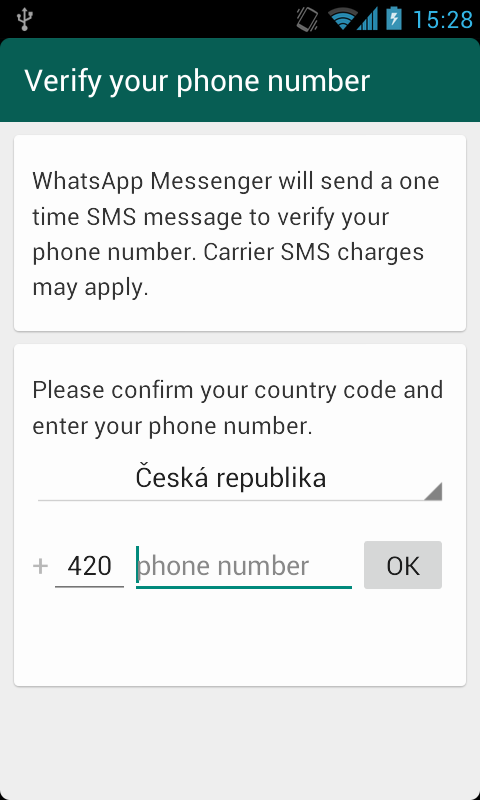
\includegraphics[width=0.4\textwidth]{whatsapp-registration.png}
	\caption{WhatsApp's registration process}
	\label{img:whatsapp_reg}
\end{figure}

Upto version 2.6.5 WhatsApp offered an alternative verification process. Instead of the user waiting for a text message, he was rather supposed to send a SMS to one of WhatsApp's phone numbers where he included his email. WhatsApp later sent verification code to the email and user verified himself with this code \cite{whatsapp-shootingthemsg}.

Serious drawbacks were found in this method in 2011 \cite{whatsapp-hijack1}. To hijack user's account attacker first opted for this method. Then using SMS spoofing service he sent SMS to WhatsApp's phone number pretending it originates from the victim. Attacker set the content of the message to an email he owned, leading to WhatsApp sending the verification code to the attacker. The attacker then simply entered the code from an email and successfully hijacked the victim's account.

Following these findings another method to bypass the registration process was published. During the registration phase WhatsApp sent a request for the verification SMS to be sent to the client in HTTP request similiar to this \cite{whatsapp-shootingthemsg}:


\begin{lstlisting}[
	caption={HTTP request to dispatch SMS},
	basicstyle=\footnotesize,
	breaklines=true
]
GET [..]?to=4915143[..]&auth=659&[..] HTTP/1.1
User-Agent: WhatsApp/2.6.4 iPhone_OS/4.3.3 Device/iPhone_4
\end{lstlisting}

The request contained the final verification code in the GET parameter. That leads to a conclusion the client created the verification code, not the server, and expected user's confirmation. An attacker could simply intercept the request, retrieved the verification code and made sure the request didn't arrive to WhatsApp's servers to let the victim unaware of malicous intentions.

Attacker then created a fake HTTP OK response to let the messenger think the request was successful and entered retrieved verification code from the intercepted request. The attacker successfully hijacked the victim's WhatsApp identity and can both send and recieve all his messages.

The author of the research notified WhatsApp developers beforehand and WhatsApp fixed this issue before the research was made public \cite{whatsapp-shootingthemsg}. To the date of writing this thesis WhatsApp doesn't offer discussed verification method anymore.


\subsubsection{Password generation}

WhatsApp uses lightly modified version of XMPP \cite{whatsapp-xmpp}. During the registration process it creates a username based on the user's phone number. In newer versions than 2.10 the password is generated on server's side \cite{whatsapp-imei}. However, older versions used the phone's IMEI  number as password \cite{whatsapp-imei}\cite{whatsapp-imei2}.

\begin{lstlisting}[caption={Pseudo-code of password generation on Android}]
md5(revert('IMEI')) 
\end{lstlisting}

Any phone number -- IMEI pair was therefore all an attacker needed to send messages on victim's behalf. Numerous applications are collecting plenty of user data and the IMEI and phone number might be among them. Any database leak with such information would lead directly to large accounts abuse.

\subsubsection{Messages encryption}

Up to version approximately 2.8 WhatsApp did not use any message encryption. The messenger used port 443 (commonly used for HTTPS) to send content, however it did not encrypt anything \cite{whatsapp-plaintext}. Using a simple network sniffer like Wireshark attacker was able to read all user's messages.

On May 2012 an application called ``WhatsAppSniffer'' had been released  \cite{whatsapp-sniffer}\cite{whatsapp-sniffer2}. It abused described flaw and enabled attacker to see victim's messages in easy and lucid user interface.


\begin{figure}[htb]
	\centering
	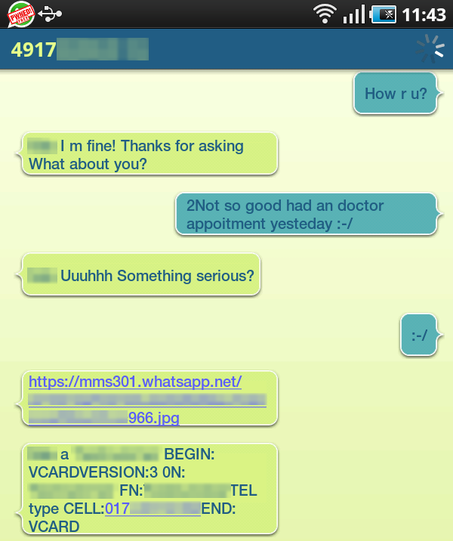
\includegraphics[width=0.4\textwidth]{whatsapp-sniffer.png}
	\caption{WhatsAppSniffer \cite{whatsapp-sniffer2}}
	\label{img:whatsapp_reg}
\end{figure}


On August 2012 WhatsApp started to use some sort of encryption. The developers did not reveal which protocol they use or any other information. Reports showed that simple message sniffing, as described in previous chapter, seized to work \cite{whatsapp-sniffernomore}. Some sources claim the  RC4 stream cipher was used for encryption \cite{whatsapp-rc4}\cite{whatsapp-rc42}.

On November 18, 2014, Open Whisper Systems, the creators behind Signal messenger, announced a partnership with WhatsApp. The partnership should have escalated into incorporating OWS' encryption protocol to WhatsApp bringing end-to-end encryption to all WhatsApp clients. Open Whisper Systems stated: \emph{``we are moving quickly towards a world where all WhatsApp users will get end-to-end encryption by default.''}. \cite{openwhisperwhatsapp}

WhatsApp confirmed this partnership, however did not comment it any further nor offered any further information. No additional information from Open Whisper Systems' side had been released as well. WhatsApp's FAQ currently only briefly states \emph{``WhatsApp communication between your phone and our server is encrypted.''}\cite{whatsapp-faq}.

On April 2015, \emph{heise.de} investigated the current state of WhatsApp's encryption. The journalists were sniffing messages using the Man-in-the-Middle technique. They showed that Android versions used end-to-end encryption and that the messages ``\emph{were encrypted according to the TextSecure protocol}''\cite{whatsapp-encstate}. However, during testing the iOS client they concluded the messages weren't protected in such manner. Finally, they concluded they are unsure whether end-to-end encryption was actually used in all cases.


\subsection{EFF's secure messaging score}

At the time of writing, WhatsApp has two points out of seven in the EFF's secure messaging scorecard \cite{eff-score}.

\begin{table}[htb]
	\centering
	\caption{WhatsApp's secure messaging score}
	\label{my-label}
	\begin{tabular}{|l|l|}
		\hline
		Are messages encrypted in transit? & \cmark \\\hline
		Are messages encrypted so the provider can not access it? & \xmark \\ \hline
		Can user verify contacts’ identities? & \xmark \\ \hline
		Are past communications secure if keys stolen? & \xmark \\ \hline
		Is the code open to independent review? & \xmark \\ \hline
		Is the cryptography design properly documented? & \xmark \\ \hline
		Has there been any recent code audit? & \cmark \\ \hline
	\end{tabular}
\end{table}


\section{Telegram}

Telegram is instant messaging service enabling users to send messages, photos, videos, stickers and files. Telegram describes itself as fast and secure solution for instant messaging and claims to be safer than WhatsApp. Compared to WhatsApp, Telegram is more cloud-based, it stores all messages on its servers and sync them with all user's devices.\cite{telegramfaq}

Nikolaj and Pavel Durov are the authors of Telegram. After leaving the  social network VK Pavel Durov founded, they focused on creating safe forms of communication leading to Telegram.

Telegram provides two modes of messaging. Besides the regular chat Telegram provides ``secret chats''. Secret chat messages are encrypted using end-to-end encryption and are not stored on Telegram's servers\cite{telegramfaq}.

\begin{figure}[htb]
	\centering
	\label{A}
	\begin{subfigure}[b]{0.4\textwidth}
		\centering
		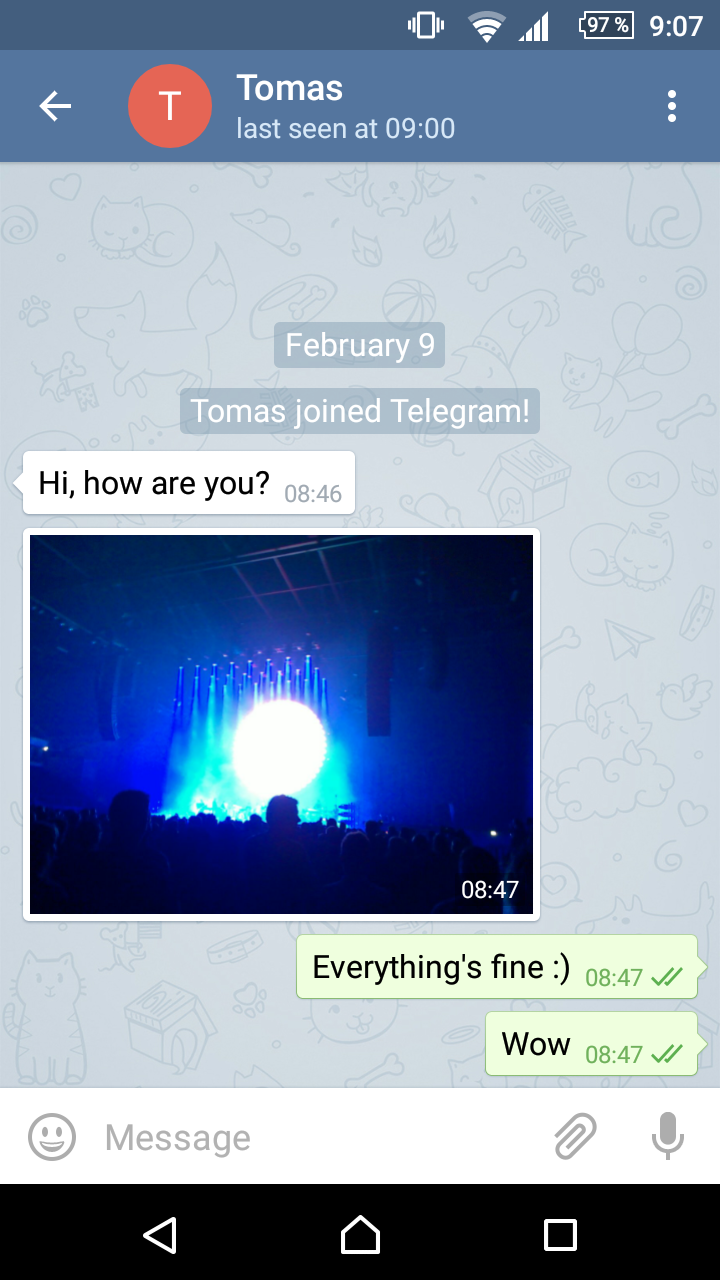
\includegraphics[width=0.9\textwidth]{telegram-regular.png}
		\caption{Regular chat}
		\label{img:telegram:regular}
	\end{subfigure}
	\hfill
	\begin{subfigure}[b]{0.4\textwidth}
		\centering
		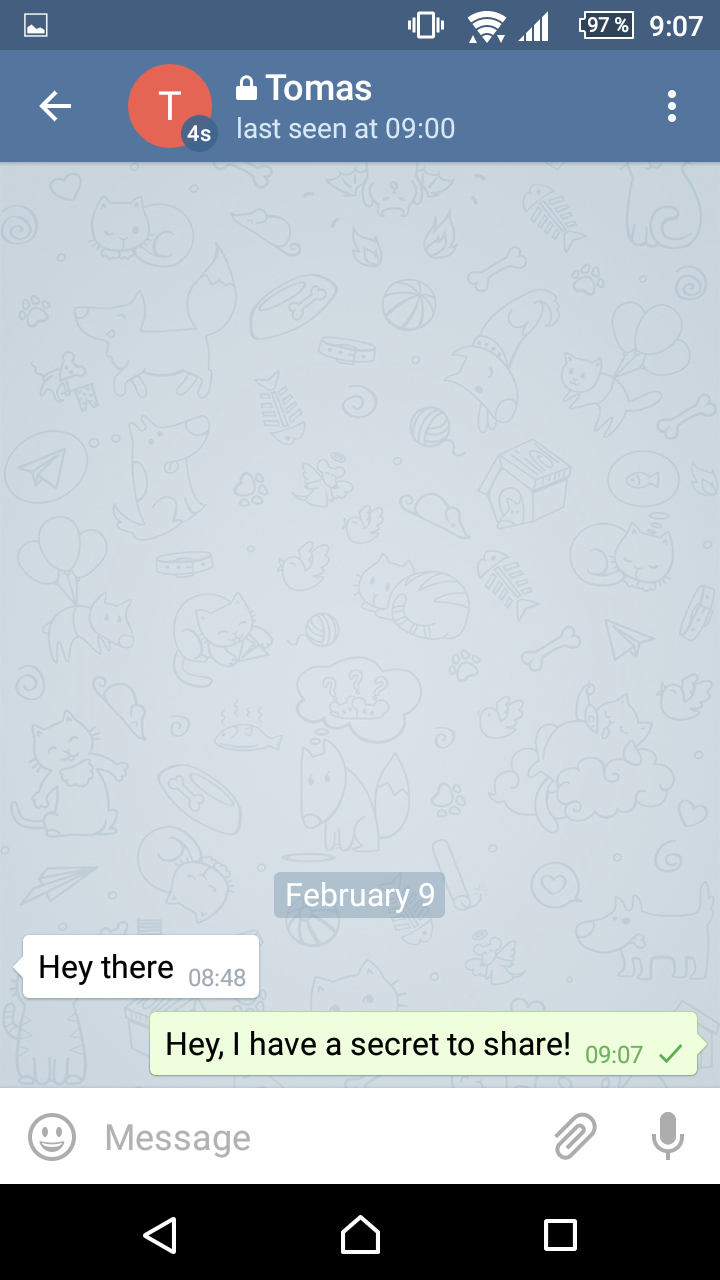
\includegraphics[width=0.9\textwidth]{telegram-secret.png}
		\caption{Secret chat}
		\label{img:telegram:secret}
	\end{subfigure}
	\caption{Telegram chat modes}
\end{figure}

Similar to WhatsApp user can contact someone using his phone number but Telegram provides classical username approach as well. User needs to know the reciepent's phone number or Telegram username in order to communicate with him.

All clients are licensed under GPLv2 or GPLv3 license, the server-side part of Telegram is closed-sourced and proprietery \cite{telegram-server}.

In 2015 Brazilian judiciary ordered WhatsApp to shut down for 48 hours. During this event, which was finally lowered to only 12 hours, Telegram welcomed 5 million new users.\cite{whatsappbrazil} It may be therefore considered as a direct competitor to WhatsApp.\footnote{Tohle je spíš taková zajímavost, tak si nejsem úplně jist na kolik to sem patří}

In May 2015 Telegram had 62 million active users \cite{telegram-users}.

\subsection{Security-related incidents}

Telegram was first released on August 14, 2013. The security-related history is thus not as broad as WhatsApp's.

\subsubsection{Possibly unsafe fundamentals}

Telegram authors decided to create a brand new encryption scheme called MTProto. In cryptography community this raised concerns and some commented the approach as ``\emph{not something that a cryptographer would use}''\cite{telegram-cryptocomm}. Some of the alleged imperfections are:

\begin{itemize}
	\item Telegram uses SHA-1 which is proven to be cryptographically broken \cite{telegram-sha1}.
	\item Telegram's authentication scheme is based on MAC-then-Encrypt approach instead of Encrypt-then-MAC.
	\item It uses IGE\footnote{Infinite Garble Extension} mode in the AES encryption which is not well known. \footnote{Pokud bych dělal Telegram, tohle je něco co by stálo za prozkoumání? Něco podobného útoku Padding Oracle. Prozkoumat ten IGE a tu autentikaci.}
\end{itemize}

Telegram FAQ contradicts it uses the primitives in a safe manner \cite{telegram-techfaq}.

\subsubsection{IND-CCA insecurity}

In Spring 2015 researchers from Aarhus University performed an independent audit of the protocol \cite{telegram-aarhus}. They concluded the encryption scheme is not IND-CCA\footnote{Indistinguishability under Chosen Ciphertext} secure, meaning any ciphertext can be altered into another ciphertext decrypting to the very same plaintext.

The researchers stressed the theoretical nature of the attack and that they ``\emph{do not see any way of turning the attack into a full plaintext-recovery attack}''\cite{telegram-aarhus}. Telegram's FAQ describes it as a minor issue unaffecting overall security. \cite{telegram-techfaq}

\subsubsection{Secret chat and Man-in-the-Middle attack}

The secret chat provides an option to display counterparty's encryption key. Telegram creates a white-blue box to visualise the key as may be seen on \ref{img:telegram-keybox}. To make sure no malicious mediator is present users are supposed to meet in person and verify the keys are identical.

\begin{figure}[htb]
	\centering
	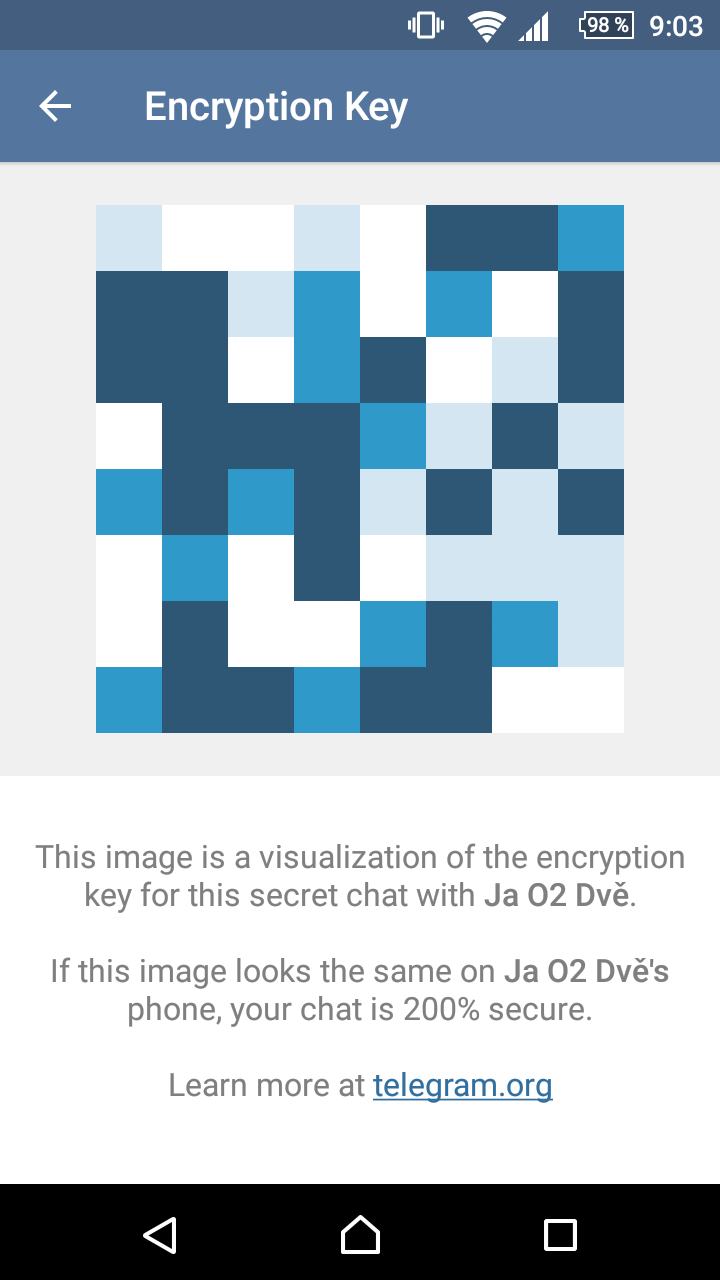
\includegraphics[width=0.4\textwidth]{telegram-keybox.png}
	\caption{Encryption key visualisation}
	\label{img:telegram-keybox}
\end{figure}

The visualisation is based on a 128-bit fingerprint of the secret key. An~article presented in January 2015 showed\cite{telegram-264} that when the attacker forces (e.g. socially engineers) both sides to initiate the secret chat, a MiM attack is possible only with $2^{64}$ operations, rather than $2^{128}$, based on the birthday paradox.\footnote{Nevím, jestli bych to měl rozepsat nějak více. Ten článek není nijak skvělý, možná stačí později, jen v případě, že si telegram vyberu?}

The article claims the attack is possible for a well financed adversary and estimates the attack to cost tens of millions USD. Telegram's FAQ addresses this issue and claimes its cost is around a trillion dollars to achieve a result in one month \cite{telegram-techfaq}.

The article as well reasons that in real-world scenario the users don't meet up to verify the key. Most of them probably ignore the verification completely, some send the image via regular chat or using another channel.

\subsubsection{Cracking Contest}

On November 4, 2014, Telegram published contest with a winning price \$300,000 for cracking its encryption. The contest became quite known in the community and probably provided a bit of advertisiment for Telegram.

The contest remained unsolved until his closure. Number of authors considered it rigged and stated that the contest does not provide any prove of Telegram's overall security whatsoever.\cite{telegramcontestfail}\cite{telegramcontestfail2}

\subsection{EFF's secure messaging score}

As mentioned Telegram has two types of messages. Telegram is therefore evaluated twice by the EFF.

\subsubsection{Telegram regular chats}

\begin{table}[htb]
	\centering
	\caption{Telegram regular chat's secure messaging score}
	\label{tab:telegram-regular-eff}
	\begin{tabular}{|l|l|}
		\hline
		Are messages encrypted in transit? & \cmark \\\hline
		Are messages encrypted so the provider can not access it? & \xmark \\ \hline
		Can user verify contacts’ identities? & \xmark \\ \hline
		Are past communications secure if keys stolen? & \xmark \\ \hline
		Is the code open to independent review? & \xmark \\ \hline
		Is the cryptography design properly documented? & \cmark \\ \hline
		Has there been any recent code audit? & \cmark \\ \hline
	\end{tabular}
\end{table}


\subsubsection{Telegram secret chats}

\begin{table}[htb]
	\centering
	\caption{Telegram secret chat's secure messaging score}
	\label{tab:telegram-secret-eff}
	\begin{tabular}{|l|l|}
		\hline
		Are messages encrypted in transit? & \cmark \\\hline
		Are messages encrypted so the provider can not access it? & \cmark \\ \hline
		Can user verify contacts’ identities? & \cmark \\ \hline
		Are past communications secure if keys stolen? & \cmark \\ \hline
		Is the code open to independent review? & \cmark \\ \hline
		Is the cryptography design properly documented? & \cmark \\ \hline
		Has there been any recent code audit? & \cmark \\ \hline
	\end{tabular}
\end{table}


\section{Signal}

Signal is a voice calling and instant messaging application developped by Open Whisper Systems. It was brought to light by the merge of two applications -- the voice calling RedPhone and the text messenger TextSecure both created by the very same company \cite{signalmerge}.

Signal is completely open-sourced including its server side. Signal was endorsed by some well-known names such as Edward Snowden \cite{signal-snowden} or Bruce Schneier \cite{signal-schneier}.

TODO

\subsection{EFF's secure messaging score}


\begin{table}[htb]
	\centering
	\caption{Signal's secure messaging score}
	\label{tab:telegram-regular-eff}
	\begin{tabular}{|l|l|}
		\hline
		Are messages encrypted in transit? & \cmark \\\hline
		Are messages encrypted so the provider can not access it? & \cmark \\ \hline
		Can user verify contacts’ identities? & \cmark \\ \hline
		Are past communications secure if keys stolen? & \cmark \\ \hline
		Is the code open to independent review? & \cmark \\ \hline
		Is the cryptography design properly documented? & \cmark \\ \hline
		Has there been any recent code audit? & \cmark \\ \hline
	\end{tabular}
\end{table}


\section{Threema}

TODO napsat cenu

Threema is paid proprietary instant messaging application. Users can send  photos, videos, voice messages, QR codes, polls and files \cite{threemahomepage}. TODO: citovani homepage?

It provides end-to-end encryption and claims to prevent collection of any metadata \cite{threemahomepage}.

Threema does not use phone numbers or usernames. It generates a random ID for user identification. Phone number and email are not required, no personal information are therefore needed.

As of June 2015, Threema had 3.5 million active users, mostly in german-speaking countries.\cite{threemausers}

\section{WeChat}

WeChat is properietary application. It was released in January 2011 and allows users to send text messages, voice messages, communicate via phone or video calls, it provides location sharing functions and other various functions \cite{wechatfeatures}.

As of August 2015, WeChat has 600 million active users, vast majority of them located in China.\cite{wechatusers}

\begin{conclusion}

Zaver TODO

\end{conclusion}

\bibliographystyle{iso690}
\bibliography{ref}

\appendix

% \printglossaries

\chapter{Contents of CD}\label{app:CDcontent}

Visualise the contents of enclosed media. Use of \verb|dirtree| is recommended. Note that directories src and text with appropriate contents are mandatory.


\begin{figure}
	\dirtree{%
		.1 readme.txt\DTcomment{the file with CD contents description}.
		.1 data\DTcomment{the data files directory}.
		.2 graphs\DTcomment{the directory of graphs of experiments}.
		.3 *.eps\DTcomment{the B/W graphs}.
		.3 *.png\DTcomment{the color g<raphs}.
		.3 *.dat\DTcomment{the graphs data files}.
		.1 exe\DTcomment{the directory with executable WBDCM program}.
		.2 wbdcm\DTcomment{the WBDCM program executable (UNIX)}.
		.2 wbdcm.exe\DTcomment{the WBDCM program executable (Windows)}.
		.1 src\DTcomment{the directory of source codes}.
		.2 wbdcm\DTcomment{the directory of WBDCM program}.
		.3 Makefile\DTcomment{the makefile of WBDCM program (UNIX)}.
		.2 thesis\DTcomment{the directory of \LaTeX{} source codes of the thesis}.
		.3 figures\DTcomment{the thesis figures directory}.
		.3 *.tex\DTcomment{the \LaTeX{} source code files of the thesis}.
		.1 text\DTcomment{the thesis text directory}.
		.2 thesis.pdf\DTcomment{the Diploma thesis in PDF format}.
		.2 thesis.ps\DTcomment{the Diploma thesis in PS format}.
	}
\end{figure}


\end{document}
